\title{Kapaliny}
\documentclass[10pt,a4paper]{article}
\usepackage[utf8]{inputenc}
\usepackage[czech]{babel}
\usepackage{amsmath}
\usepackage{amsfonts}
\usepackage{amssymb}
\usepackage{chemfig}
\usepackage{geometry}
\usepackage{wrapfig}
\usepackage{graphicx}
\usepackage{floatflt}
\usepackage{hyperref}
\usepackage{fancyhdr}
\usepackage{tabularx}
\usepackage{makecell}
\usepackage{csquotes}
\usepackage{footnote}
\usepackage{movie15}
\MakeOuterQuote{"}

\renewcommand{\labelitemii}{$\circ$}
\renewcommand{\labelitemiii}{--}
\newcommand{\ra}{$\rightarrow$ }
\newcommand{\x}{$\times$ }
\newcommand{\lp}[2]{#1 -- #2}
\newcommand{\timeline}{\input{timeline}}


\geometry{lmargin = 0.8in, rmargin = 0.8in, tmargin = 0.8in, bmargin = 0.8in}
\date{\today}
\author{Jakub Rádl}

\makeatletter
\let\thetitle\@title
\let\theauthor\@author
\makeatother

\hypersetup{
colorlinks=true,
linkcolor=black,
urlcolor=cyan,
}



\begin{document}
\maketitle
\tableofcontents
\begin{figure}[b]
Toto dílo \textit{\thetitle} podléhá licenci Creative Commons \href{https://creativecommons.org/licenses/by-nc/4.0/}{CC BY-NC 4.0}.\\ (creativecommons.org/licenses/by-nc/4.0/)
\end{figure}
\newpage

\section{Struktura a vlastnosti kapalin}

\subsection{Povrchové napětí}
$E = \sigma S$

\paragraph{Exp.: }
\begin{itemize}
\item dvacetník plave na hladině i když má vyšší hustotu, než voda
\end{itemize}

\paragraph{Povrchové napětí}\mbox{} \\ \mbox{} \\
\begin{wrapfigure}{l}{0.4\textwidth}
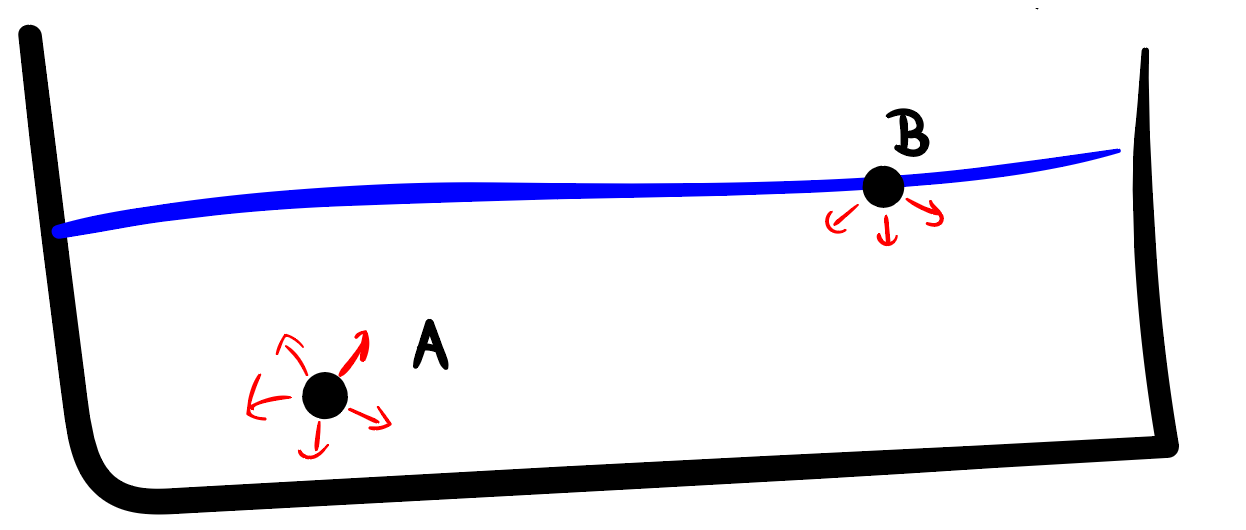
\includegraphics[width=0.4\textwidth]{pictures/007.png}
\vspace{-40px}
\end{wrapfigure}

\begin{itemize}
\item molekula na hladině má cca polovinu vazeb jako uprostřed
\item aby se molekula dostala na povrch, je potřeba přetrhat některé vazby -- vykonat práci
\item na zvětšení povrchu je potřeba vykonat $\sigma S$ práce
\end{itemize} \mbox{} \\

\paragraph{Př.: Jak se změní energie bubliny, změní li se její poloměr na polovinu?}
\begin{itemize}
\item $E = \sigma S$; $S_{koule} = 4\pi r$
\item $\Delta E = E_1 - E_2 = 4 \sigma \pi r^2 - 4 \sigma \pi (\frac{r}{2})^2 = 3 \sigma \pi r^2$
\item $r_{bublina} = 2$cm, $\sigma_{voda} = 40$mJm$^{-2}$
\item $\Delta E = 3 \cdot 0.04 \cdot 0.02^2 \cdot \pi = 0.000048 \pi$J 
\end{itemize}

\paragraph{Praxe: Kapilární jevy}
\begin{itemize}
\item kapalina smáčí látku (je přitahována)
\item tenká trubička / porézní materiál
\item povrch kapaliny se zmenší zaplnění dutin \ra energeticky výhodné
\item rostliny nasávají vodu pomocí kapilárních jevů
\end{itemize}

\paragraph{Praxe: Hydrofobní úprava}
\begin{itemize}
\item úprava povrchu, aby voda nesmáčela látku
\item impregnace povrchu
\item gore-tex -- tenká vrstva teflonu s malými póry
\end{itemize}

\subsection{Teplotní roztažnost}
\begin{itemize}
\item délková roztažnost: $\Delta l = \Delta T \alpha l_0$
\item $l = l_0 + \Delta l = l_0 + \Delta T \alpha l_0 = l_0(1+\alpha \Delta T)$
\item Ocel: $\alpha = 1.15 \cdot 10^{-5}$ K$^{-1}$
\end{itemize}

\paragraph{Praxe:}
\begin{itemize}
\item bimetal
\item mosty, koleje, dráty
\end{itemize}

\subsection{Objemová roztažnost:}
\begin{itemize}
\item $\Delta V = V_0 \cdot \beta \cdot \Delta T$
\item $\beta \doteq 3\alpha$
\item Líh: $\beta = 11\cdot 10^{-4}$ K$^{-1}$
\end{itemize}

\paragraph{Praxe:}
\begin{itemize}
\item teploměr, termostat, voda -- anomálie
\end{itemize}

\end{document}